\section{Studio attraverso il prisma}
In primo luogo abbiamo fatto incidere il fascio collimato, proveniente da una lampada a Hg, su una delle facce ottiche del prisma e abbiamo ruotato l'oggetto analizzatore fino ad osservare l'angolo di inversione.
Prima di procedere è stato però necessario misurare l'angolo al vertice del prisma, ovvero l'angolo tra le due facce ottiche, riportadone la base su un foglio e osservando la congruenza di tutti i lati a meno di un errore di un millimetro.
L'angolo al vertice è risultato, quindi, essere di $\alpha$\,=\,60°.
Preso come zero l'angolo di allineamento, ovvero l'angolo per cui le due lenti permettevano una visione nitida del raggio luminoso, abbiamo proceduto misurando l'angolo di minima deviazione per ogni linea distinguibile:

\begin{table}[h!]
    \centering
    \begin{tabular}{cc}
    \toprule
    $\vartheta$ & angolo totale $\delta$ (rad)\\
    \midrule
    90°	0' &0,854\\
    90°	20' &0,860\\
    90°	40' &0,866\\
    91°	20' &0,877\\
    91°	23' &0,878\\
    92°	24' &0,896\\
    93°	20' &0,912\\
    93°	35' &0,916\\
\bottomrule
    \end{tabular}
    \caption{}
    \label{tab:my_label}
\end{table}
\noindent
%io anzichè mettere il numero della linea metterei più il range di colore

Da questi valori abbiamo ricavato l'indice di rifrazione per ogni lunghezza d'onda attraverso la formula:

\begin{equation}
n=\dfrac{\sin\left(\dfrac{\delta+\alpha}{2}\right)}{\sin\left(\dfrac{\alpha}{2}\right)}
\label{eq 2}
\end{equation}
Dall'Eq. \ref{eq 2} si può stimare l’incertezza su $n$ propagando l'errore sull'angolo
$$
\sigma^2_n = \left|\dfrac{\partial n}{\partial\delta} \right|^2\sigma^2_{\delta}
$$
\begin{equation}
    \sigma_{n}^{2}=\frac{1}{4}\left(\frac{1}{\sin ^{2}\left(\frac{\alpha}{2}\right)}-n^{2}\right)\sigma_{\delta}^{2}
\end{equation}
La seguente tabella mostra i risultati ottenuti

\begin{table}[h!]
    \centering
    \begin{tabular}{ccc}
    \toprule
    \textit{n} & $\lambda (\angstrom)$& $\sigma_n$ ($10^{-5}$)\\
    \midrule
    1,6276	&4046,56 &  94\\
    1,6309	&4339,22 &  94\\
    1,6343	&4347,49 &  93\\
    1,6410	&4358,33 &  91\\
    1,6415	&5460,73 &  91\\
    1,6515	&5769,60 &  89\\
    1,6607	&5790,66 &  87\\
    1,6631	&7081,90 &  86\\
\bottomrule
    \end{tabular}
    \caption{Indici di rifrazione con relativo errore}
\end{table}
\noindent
Infine abbiamo realizzato un fit lineare dei parametri al fine di stimare i coefficienti della legge di Cauchy al secondo ordine. I risultati del fit sono riportati di seguito.
\begin{figure}[h!]
    \centering
    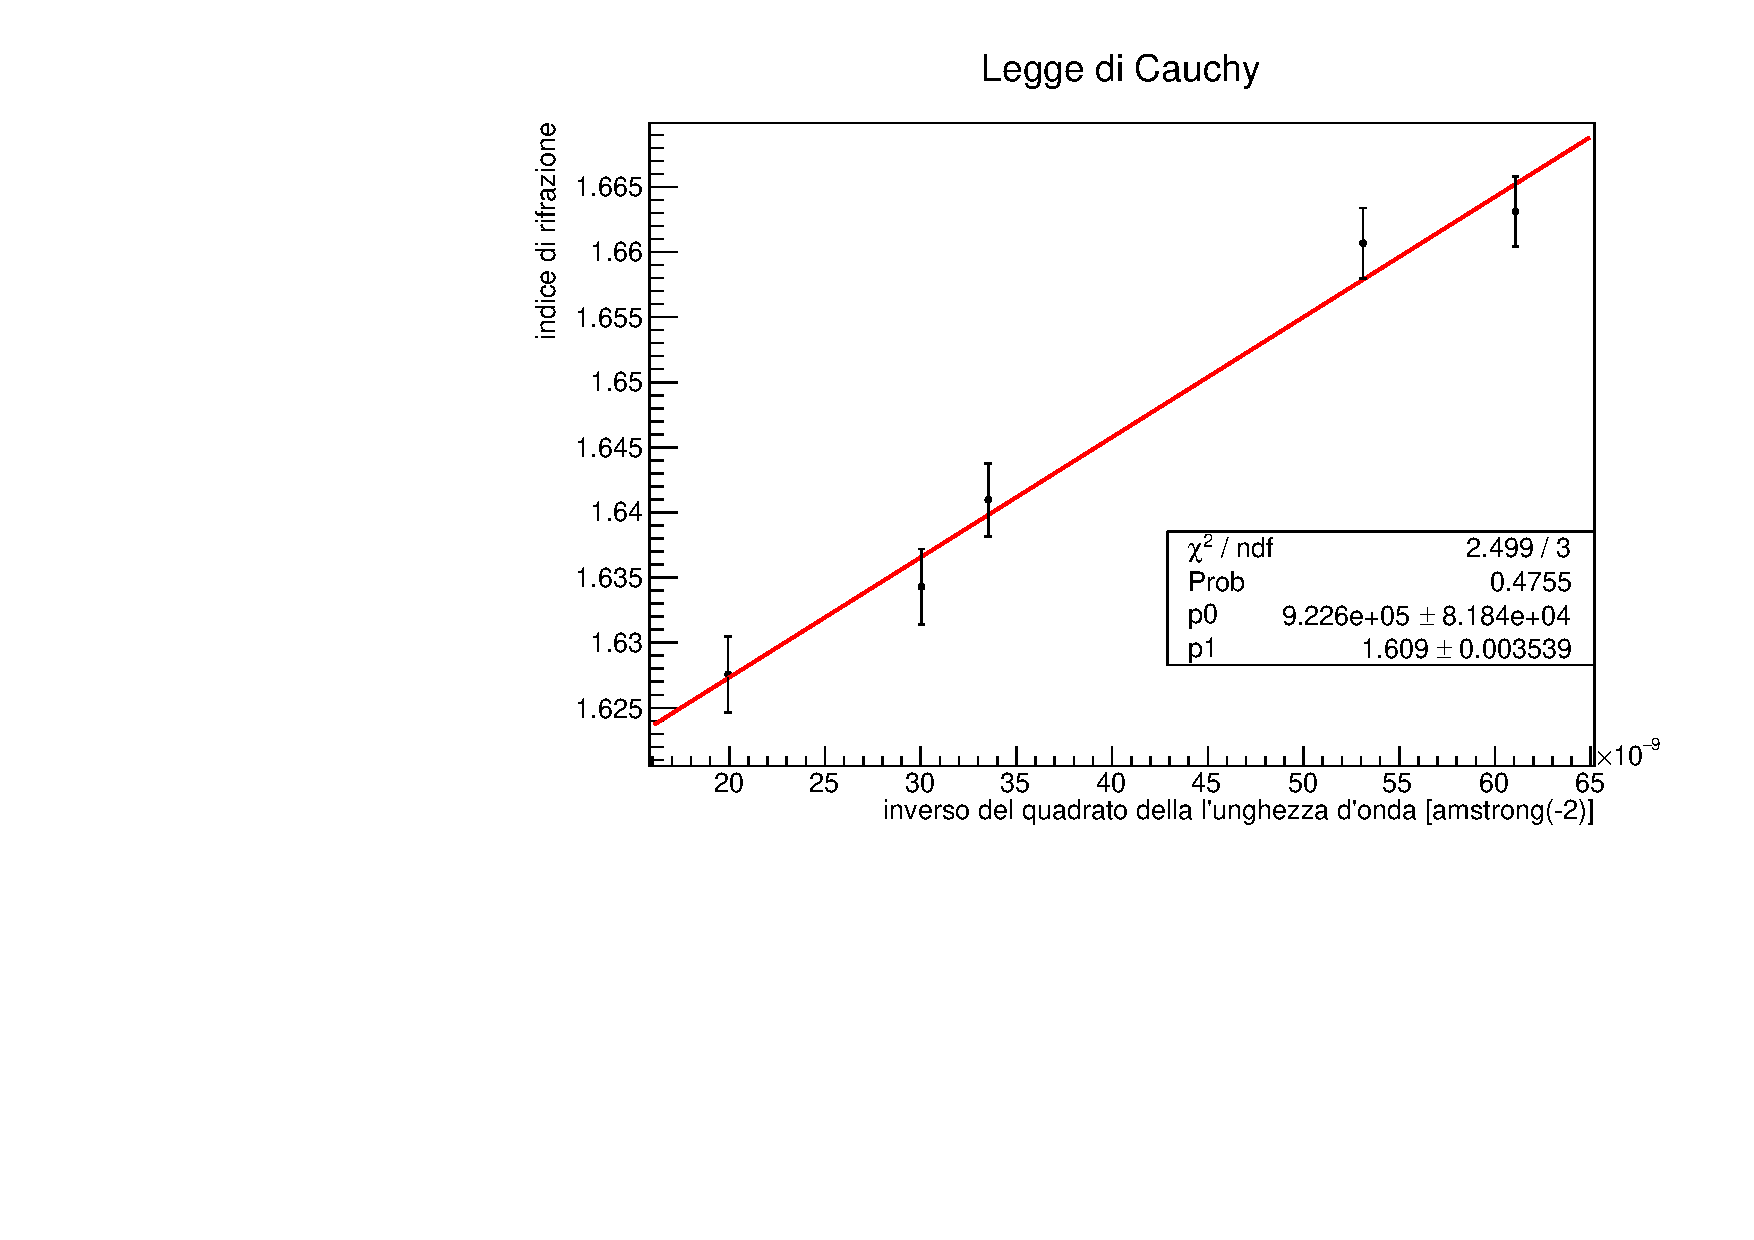
\includegraphics[scale=.65]{Immagini/Legge Cauchy.pdf}
    \caption{Il parametro A della legge di Cauchy qui è riportato come p1, mentre B come p0.}
\end{figure}

\noindent
Avendo una probabilità di $\chi^2$ maggiore di $0.05$, il fit viene considerato accettabile, la legge di Cauchy viene considerata verificata ed i parametri che la descrivono vengono stimati come:
$$
A = 1,609 \pm 0,003\qquad B= (92,26\pm 8,184)\times 10^{4}\,\angstrom^{-2}   \qquad \rho_{AB}= 1.2527\times 10^{-5}
$$